\let\negmedspace\undefined
\let\negthickspace\undefined
\documentclass[journal,12pt,twocolumn]{IEEEtran}
\usepackage{cite}
\usepackage{amsmath,amssymb,amsfonts,amsthm}
\usepackage{algorithmic}
\usepackage{graphicx}
\usepackage{textcomp}
\usepackage{xcolor}
\usepackage{txfonts}
\usepackage{listings}
\usepackage{enumitem}
\usepackage{mathtools}
\usepackage{gensymb}
\usepackage{comment}
\usepackage[breaklinks=true]{hyperref}
\usepackage{tkz-euclide} 
\usepackage{listings}
\usepackage{gvv}                                        
\def\inputGnumericTable{}                                 
\usepackage[latin1]{inputenc}                                
\usepackage{color}                                            
\usepackage{array}                                            
\usepackage{longtable}                                       
\usepackage{calc}                                             
\usepackage{multirow}                                         
\usepackage{hhline}                                           
\usepackage{ifthen}                                           
\usepackage{lscape}

\newtheorem{theorem}{Theorem}[section]
\newtheorem{problem}{Problem}
\newtheorem{proposition}{Proposition}[section]
\newtheorem{lemma}{Lemma}[section]
\newtheorem{corollary}[theorem]{Corollary}
\newtheorem{example}{Example}[section]
\newtheorem{definition}[problem]{Definition}
\newcommand{\BEQA}{\begin{eqnarray}}
\newcommand{\EEQA}{\end{eqnarray}}
\newcommand{\define}{\stackrel{\triangle}{=}}
\theoremstyle{remark}
\newtheorem{rem}{Remark}

\begin{document}
\bibliographystyle{IEEEtran}

\vspace{3cm}

\title{}
\author{EE23BTECH11047 - Deepakreddy P
}
\maketitle
\newpage
\bigskip

\noindent \textbf{17} \quad 
If a, b, c, d are in G.P, prove that 
$ \brak{a^{n} + b^{n}},\brak{b^{n} + c^{n}},\brak{c^{n} + d^{n}} $ are in G.P and find the Z transform of General term of G.P.\\
\solution

\begin{center}
    \begin{table}[ht]
        \setlength{\arrayrulewidth}{0.3mm}
\setlength{\tabcolsep}{12pt}
\renewcommand{\arraystretch}{1.5}


\begin{center}
\caption{Input Parameters}
\begin{tabular}{|c|c|}

\hline
 {Symbol}&{Remarks}\\
\hline
$x(0) $ & $a$ \\
\hline
$x(1) $ & $b$ \\
\hline
$x(2) $ & $c$ \\
\hline
$x(3) $ & $d$ \\
\hline
$r$ & ratio of G.P a,b,c....\\
\hline
$r_1$ & ratio of G.P $a^n + b^n,b^n + c^n,....$\\
\hline
$X(z)$ & z transform of G.P a,b,c....\\
\hline
$Y(z)$ & z transform of G.P $a^n + b^n,b^n + c^n,....$\\
\hline

\end{tabular}
\end{center}

    \end{table}
\end{center}

\begin{align} 
 &=\frac{x\brak{1}^n + x\brak{2}^n}{x\brak{0}^n + x\brak{1}^n}  \\
&= \frac{\brak{x\brak{0}r^1}^n + \brak{x\brak{0}r^2}^n}{\brak{x(0)r^0}^n + \brak{x\brak{0}r^1}^n}\\
&= \frac{x\brak{0}^n r^n \brak{1 + r^n}}{x\brak{0}^n \brak{1 + r^n}} \\
&= \frac{x(0)^n r^{2n} \brak{1 + r^n}}{x\brak{0}^n r^n \brak{1 + r^n}}\\
&= \frac{\brak{x\brak{0} r^2}^n + \brak{x\brak{0} r^3}^n}{\brak{x\brak{0} r^1}^n + \brak{x\brak{0} r^2}^n}\\
&= \frac{x\brak{2}^n + x\brak{3}^n}{x\brak{1}^n + x\brak{2}^n}
\end{align}
Hence proved they are in in G.P

\begin{align}
    x\brak{n} &= x\brak{0}r^{n} u\brak{n}\\
    X\brak{z} &= \frac{x\brak{0}}{1-rz^{-1}}, \quad |z|>|r|
\end{align}
\newpage
\begin{figure}[h]
   \centering
   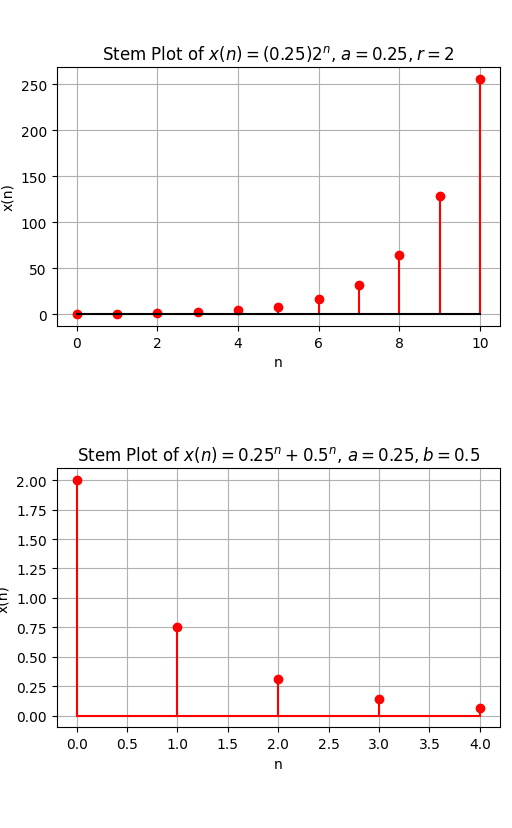
\includegraphics[width=1\columnwidth]{figs/gp.png}
   \caption{Plot of x(n) vs n}
   \label{fig: Stem plot of x(n)}
\end{figure}





\end{document}

